\chapter{Geometry of the Expanding Universe}

These notes follow Leonard Susskind's first cosmology lecture as closely as possible in both argument and pace. The transcript, together with selected blackboard frames preserved through LazyingArt LLC and Video2Book, lets us keep the order of discovery clear: first a toy expanding universe, then Hubble's law, then the metric of space, and only then the metric of spacetime. The lecture is deliberately geometry-first. Newtonian cosmology, Einsteinian dynamics, and the full Friedmann--Robertson--Walker package are promised for later. Here we are interested in a simpler question: what does it mean, geometrically, to say that the universe expands?

\section{Geometry First, Dynamics Later}

Susskind begins by declining to tell the whole history of cosmology. We are to get straight to the point, and the point is the expanding universe and its geometry. That opening is not merely rhetorical. It tells us why this chapter begins with idealized lines, grids, and metrics, and not with Einstein's equations.

The roadmap is brief but important. We will study the geometry of expanding universes first and leave the physics of expansion for later. Newtonian \(F=ma\) cosmology will come next, and only after that will geometry and dynamics be fused into the full FRW description. The present lecture therefore asks us to be disciplined: for now we describe the universe; we do not yet ask what drives the description.

\section{Comoving Coordinates and the One-Dimensional Expanding Line}

We begin with the simplest possible space: one-dimensional space, \emph{space, not spacetime}. Take an infinite line, place equally spaced galaxies on it, and label the galaxies by a coordinate \(x\). The first conceptual point is that the coordinate is not yet a measured distance. It is a tag attached to a galaxy, and it moves with the galaxy if the universe expands or contracts. One may think of \(x\) as the name of the galaxy.

\begin{figure}
\centering
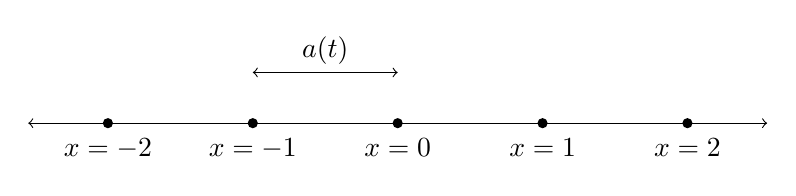
\begin{tikzpicture}[scale=0.92]
\draw[<->] (-5.1,0) -- (5.1,0);
\foreach \x/\lab in {-4/-2,-2/-1,0/0,2/1,4/2}{
  \fill (\x,0) circle (2pt);
  \node[below] at (\x,-0.08) {$x=\lab$};
}
\draw[<->] (-2,0.7) -- (0,0.7);
\node at (-1,1.0) {$a(t)$};
\end{tikzpicture}
\caption{A one-dimensional universe of equally spaced galaxies. The labels \(x=-2,-1,0,1,2\) are comoving coordinates; the neighboring physical separation is the scale factor \(a(t)\).}
\end{figure}

Suppose the distance from the galaxy called \(x=0\) to the galaxy called \(x=1\) is some measured quantity \(a\). Then the distance between any two galaxies is the coordinate difference multiplied by this common spacing:
\begin{equation}
d=a\,\Delta x.
\end{equation}
This is the first mathematical move that matters. The coordinate difference \(\Delta x\) is not itself the physical distance. It only records which two galaxies we have chosen. The scale factor \(a\) converts a comoving label difference into a true geometric separation.

Now we imagine the line as an elastic thread. Two giants pull on its ends and stretch it or let it contract. The labels remain attached to the galaxies, but the neighboring physical spacing changes. Thus \(a\) becomes time-dependent:
\begin{equation}
d(t)=a(t)\,\Delta x.
\end{equation}
At this stage homogeneity means simply that neighboring galaxies are equally spaced everywhere. The common spacing may still vary with time.

This is already enough structure to say something nontrivial. We have a universe in which points carry fixed comoving labels while the physical distance between them changes. That is the raw material from which the rest of the lecture is built.

\section{From the Scale Factor to Hubble's Law}

We now calculate the rate at which the distance between two fixed galaxies changes. The word fixed matters: we keep the same pair of galaxies, so \(\Delta x\) is constant in time. Differentiating \(d=a\,\Delta x\) gives
\begin{align}
\dot d &= \dot a\,\Delta x \\
       &= \frac{\dot a}{a}\,a\,\Delta x \\
       &= \frac{\dot a}{a}\,d.
\end{align}
This is Hubble's law in its cleanest form. If we define
\begin{equation}
H(t)\equiv \frac{\dot a}{a},
\end{equation}
then the law reads
\begin{equation}
\dot d = H(t)\,d.
\end{equation}

Susskind follows the standard historical language and says ``Hubble constant,'' but he immediately pauses to correct the impression that the name gives. The quantity is constant in space, not in time. It is the same for every galaxy at a given moment, but in general it evolves with the universe. So in the notes we should hear his warning and keep in mind that \(H(t)\) is really the Hubble parameter.

The physical content comes next. Galaxies farther away recede faster. But the argument does not pick out a center. Nothing in the formula privileges \(x=0\), \(x=1\), or any other point. The law concerns relative separation, and it is the same everywhere. The expanding universe described here is therefore not a blast from one distinguished place.

Only after deriving the law does the lecture turn outward toward observation. If Alice and Bob exchange light signals while moving apart, the received light is redshifted. The faster the recession, the greater the redshift. Spectral lines therefore offer a way to estimate recession speed. Distance is harder, but Hubble used rough observational surrogates such as brightness and angular size. His plot was not a perfect straight line. It was noisy, with large scatter, and his original distances were badly misestimated. But the geometric principle was right: recession speed is proportional to distance.

A second caution is briefly raised and deferred. If \(d\) is large enough, the formula predicts \(\dot d>1\) in units with \(c=1\). Susskind flags that as important, but leaves the resolution for later lectures.

\subsection{Question \& Answer}

\paragraph{Question.} Does \(v=Hd\) mean that a given pair of galaxies must be accelerating, simply because the distance \(d\) is increasing?

\paragraph{Answer.} No. The law says that velocity increases with distance at a given moment. It does \emph{not} by itself say whether the velocity of one fixed pair increases with time. That depends on how \(a(t)\) behaves.

If
\begin{equation}
a(t)=\alpha t,
\end{equation}
then neighboring galaxies separate at constant speed:
\begin{equation}
\dot d=\alpha\,\Delta x.
\end{equation}
The recession speed depends on the pair we choose, but it does not change with time.

If instead
\begin{equation}
a(t)=\beta t^2,
\end{equation}
then
\begin{equation}
\dot d=2\beta t\,\Delta x,
\end{equation}
so the recession speed of a fixed pair increases with time.

And if
\begin{equation}
a(t)=\gamma \log t,
\end{equation}
then
\begin{equation}
\dot d=\frac{\gamma}{t}\,\Delta x,
\end{equation}
so the recession speed decreases with time.

Thus Hubble's law is always true as a function of distance. Whether the universe is accelerating or decelerating is a second question, encoded in the detailed time dependence of \(a(t)\). Susskind uses exactly these elementary examples to separate the two issues before moving on.

\section{Higher Dimensions, Isotropy, and Homogeneity}

At this point the lecturer says, in effect, that there is nothing especially one-dimensional about the argument. So let us widen the stage. In two dimensions we imagine a square grid of galaxies. Each galaxy carries two labels, \((x,y)\), and these labels again move with the galaxies rather than measuring physical distance directly.

Before writing the distance formula, the lecture asks a natural question: why should the spacing along the \(x\)-direction be the same as the spacing along the \(y\)-direction? The answer is not abstract formalism; it is observation. If the galaxy distribution were systematically more crowded along one axis than another, we would see that anisotropy in the sky. On sufficiently large scales, we do not. That empirical fact is what motivates using the same scale factor in all spatial directions.

\begin{figure}
\centering
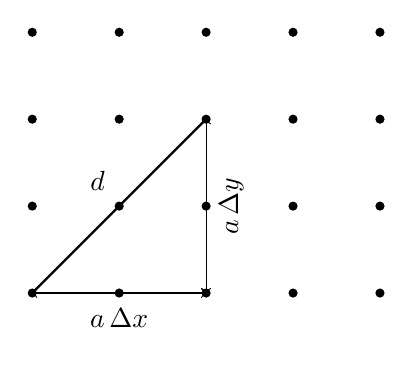
\begin{tikzpicture}[scale=0.92]
\foreach \x in {0,1,2,3,4}{
  \foreach \y in {0,1,2,3}{
    \fill (1.2*\x,1.2*\y) circle (1.8pt);
  }
}
\draw[<->] (0,0) -- (2.4,0);
\node at (1.2,-0.35) {$a\,\Delta x$};
\draw[<->] (2.4,0) -- (2.4,2.4);
\node[rotate=90] at (2.75,1.2) {$a\,\Delta y$};
\draw[thick] (0,0) -- (2.4,2.4);
\node at (0.9,1.55) {$d$};
\end{tikzpicture}
\caption{A two-dimensional comoving grid. The lecture uses such a grid only as a geometric idealization, but it makes the roles of homogeneity, isotropy, and the Pythagorean theorem transparent.}
\end{figure}

With that understood, the distance between two galaxies separated by \(\Delta x\) and \(\Delta y\) is found from the Pythagorean theorem:
\begin{equation}
d=a\sqrt{(\Delta x)^2+(\Delta y)^2}.
\end{equation}
And in three dimensions the extension is immediate:
\begin{equation}
d=a\sqrt{(\Delta x)^2+(\Delta y)^2+(\Delta z)^2}.
\end{equation}
For a fixed pair of galaxies the coordinate differences are constant, so differentiation once again gives
\begin{equation}
\dot d=\frac{\dot a}{a}\,d.
\end{equation}
The Hubble law survives unchanged.

Now the lecture names the two symmetries that have been guiding the construction. Homogeneity means sameness from place to place. Isotropy means sameness from direction to direction. Susskind is careful not to over-polish this into textbook dogma. The universe is not homogeneous on the scale of a galaxy, nor even on modest astronomical scales. It is not perfectly isotropic when we look within the Milky Way. But after averaging over many galaxies, the large-scale sky looks roughly the same in every direction, and that is the working content of the cosmological principle at this stage.

\section{Why the Scale Factor Is a Bookkeeping Device, and Why the Metric Matters}

The lecture next doubles back to a subtle point that is easy to miss if we move too fast. If \(H=\dot a/a\) is what enters Hubble's law, does the overall numerical value of \(a\) by itself have any physical meaning? Susskind's answer is no. The scale factor is, in part, a bookkeeping device. One may redefine it by a constant multiple without changing the observable Hubble law.

If we introduce a new scale factor \(b\) by
\begin{equation}
b=3a,
\end{equation}
then
\begin{equation}
\frac{\dot b}{b}=\frac{3\dot a}{3a}=\frac{\dot a}{a}.
\end{equation}
So the overall normalization of the scale factor is conventional. What matters physically is how it changes, not its absolute magnitude. This is the lecture's answer to the question about the ``initial value'' of \(a\): one may choose units or normalization freely, but the ratio \(\dot a/a\) does not care.

Only after that clarification does Susskind turn from kinematics to geometry proper. For neighboring points we replace \(\Delta x\) by \(dx\). Then the physical distance between neighboring points is
\begin{equation}
ds=a\,dx,
\end{equation}
and therefore
\begin{equation}
ds^2=a^2\,dx^2.
\end{equation}
This is now a spatial metric. In one dimension the coefficient of \(dx^2\) is simply
\begin{equation}
g_{xx}=a^2.
\end{equation}
So an expanding universe can be described by saying that the spatial metric itself is time-dependent.

The lecture then pushes one step further and asks for the spacetime metric. Proper time must include both the time separation and the physical spatial separation. Since the physical spatial distance is \(a\,dx\), the natural one-dimensional spacetime line element becomes
\begin{equation}
d\tau^2=dt^2-a^2(t)\,dx^2.
\end{equation}
For a comoving observer, \(dx=0\), so proper time reduces to ordinary time. For an object moving across the comoving grid, the spatial term contributes in the usual relativistic way.

The frame below is worth keeping precisely because it shows how the lecture makes the transition on the board: spacetime sketch on the left, cleaned line element in the middle, metric notation on the right.

\begin{figure}
\centering

\includegraphics[width=0.82\textwidth]{lecture_01_figure_02.png}

\vspace{1em}

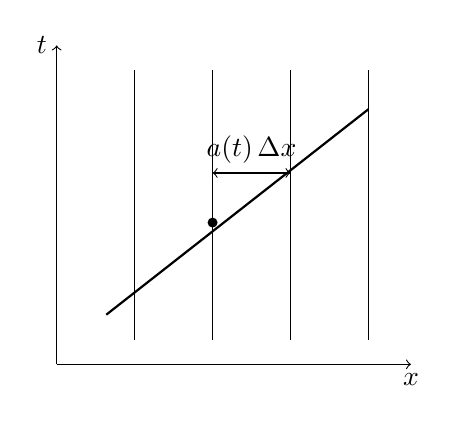
\begin{tikzpicture}[scale=0.9]
\draw[->] (0,0) -- (0,4.5);
\node[left] at (0,4.5) {$t$};
\draw[->] (0,0) -- (5.0,0);
\node[below] at (5.0,0) {$x$};

\foreach \x in {1.1,2.2,3.3,4.4}{
  \draw (\x,0.35) -- (\x,4.15);
}

\draw[thick] (0.7,0.7) -- (4.4,3.6);
\fill (2.2,2.0) circle (2pt);

\draw[<->] (2.2,2.7) -- (3.3,2.7);
\node[above] at (2.75,2.7) {$a(t)\,\Delta x$};
\end{tikzpicture}
\caption{Expanding-universe spacetime sketch and metric evidence. The screenshot preserves the lecture's board layout; the redraw isolates the comoving worldlines and the fixed-time spatial separation.}
\end{figure}

In three spatial dimensions the board writing is only partly visible, so the standard clean form should be read as a cautious reconstruction supported by both the transcript and the frame:
\begin{equation}
d\tau^2=dt^2-a^2(t)\bigl(dx^2+dy^2+dz^2\bigr).
\end{equation}
Likewise, the matrix on the right side of the board is partly occluded, but the intended diagonal form is clear enough to write it carefully as
\begin{equation}
g_{\mu\nu}=\mathrm{diag}\bigl(1,-a^2,-a^2,-a^2\bigr).
\end{equation}
The off-diagonal terms vanish:
\begin{equation}
g_{tx}=g_{ty}=g_{tz}=0,
\end{equation}
which is the lecture's way of saying that in this simple ansatz there are no mixed \(dt\,dx\)-type terms.

\subsection{Question \& Answer}

\paragraph{Question.} Is \(dx\) a physical distance, or only a comoving label?

\paragraph{Answer.} It is only a comoving label interval. The physical distance is \(ds=a\,dx\). The clean way to think about it is exactly the way Susskind phrases it: draw a coordinate mesh through the galaxies and decree that the mesh follows them. Then \(\Delta x\) between two chosen galaxies stays fixed by construction, while the measured distance between them changes because the scale factor changes. One may place the units in \(x\), or in \(a\), or split them between the two; that is convention. What is not conventional is the product \(a\,dx\), and what is especially invariant is the ratio \(\dot a/a\).

The lecture also pauses here over another convention. The coefficient of \(dt^2\) has been set equal to \(1\), and Susskind remarks that if that coefficient depended only on time, one could absorb it into a redefinition of the time variable. Similarly, he adopts units with \(c=1\). None of that changes the main point: expansion is the time dependence of the spatial components of the metric.

We are still not doing dynamics. One could now ask what energy-momentum tensor inserted into Einstein's equations would produce this metric, but the lecture explicitly postpones that. Geometry first, dynamics later.

\section{What We Know, What We Assume, and What the Horizon Hides}

With the metric in hand, Susskind makes what he calls a slightly finer distinction. Homogeneity means the metric coefficients do not depend on spatial position. Isotropy means the spatial directions are treated alike. In the diagonal metric above, the fact that the coefficients do not depend on \(x\), \(y\), or \(z\) is the metric statement of homogeneity. The fact that the three spatial coefficients are equal is the metric statement of isotropy.

\subsection{Question \& Answer}

\paragraph{Question.} What exactly do homogeneity and isotropy buy us, and how are they related?

\paragraph{Answer.} They buy us an enormous simplification. Homogeneity says the metric can depend on time but not on where we are in space. Isotropy says the \(x\)-, \(y\)-, and \(z\)-directions must enter in the same way. The two ideas are not identical: a universe may be homogeneous and still have a preferred direction. But isotropy about every point forces homogeneity. That is why the lecture treats them as distinct concepts that are closely related rather than identical principles.

The lecture then becomes deliberately cautious. The universe is not exactly homogeneous at small scales, nor exactly isotropic in every local observation. A farmer's field provides the analogy: on one scale it looks homogeneous, on a smaller scale it plainly does not, and on a scale larger than the whole field it again ceases to look homogeneous. Cosmology is similar. On scales of galaxies the universe is highly structured; only after averaging over much larger scales does the rough uniformity emerge.

That caution widens into a discussion of the horizon. We do not see the whole universe. More strongly, we do not even see all of the universe that could ever in principle affect us. Beyond the observable region we do not know whether homogeneity and isotropy continue to hold. There may be indirect clues, but the lecture insists that the horizon is an ultimate barrier to direct knowledge.

This is why the cosmological principle is both fruitful and modest. It is a powerful empirical approximation on the scales astronomy can probe, but it is not a metaphysical guarantee about arbitrarily large scales.

\section{Closed and Bounded Universes: The Circle Model}

Only after laying out the flat expanding picture does the lecture pivot to closed geometries. The order matters. We are now varying the global shape of space while preserving the local logic of comoving labels, scale factor, and Hubble flow.

The first step is to reject the wrong bounded models. A line segment has finite extent, but it comes with distinguished endpoints. A cube with walls is finite, but it violates both homogeneity and isotropy: observers near a wall see something different from observers far from a wall, and even an observer at the center sees different things in different directions. So boundedness, if the universe is to remain homogeneous and isotropic, cannot mean a box with edges.

The right idea is bounded without boundary. Susskind first gestures toward the surface of a sphere, not the interior of a ball. A two-dimensional creature confined to the surface of a featureless sphere finds every place and every direction locally the same, yet the world is finite. That is the model of boundedness he wants. He then reduces the example to one dimension, because the algebra is simpler there: life on a circle.

In one dimension isotropy means left and right are equivalent. A circle has exactly that feature. The convenient coordinate is the angle \(\theta\), measured in radians. We choose one galaxy and call it \(\theta=0\), then label every other point by an angular coordinate. A point just to the ``left'' of the origin may be described by a small negative angle or, equivalently, by an angle just short of \(2\pi\). That periodicity is part of the geometry and not a side remark.

There is also a brief notational wobble in the lecture that is worth preserving in cleaned form. Susskind momentarily hesitates over whether to call the whole circumference the scale factor or to write it as \(2\pi\) times a radius-like quantity. The cleaner convention, and the one we keep, is
\begin{equation}
L=2\pi a,
\end{equation}
where \(L\) is the total distance around the circle and \(a\) is the radius-like parameter of the external plotting circle.

Then, for a small angular separation \(\Delta\theta\), the physical arc length is
\begin{equation}
d=a\,\Delta\theta.
\end{equation}
Passing to infinitesimals gives the local metric
\begin{equation}
ds=a\,d\theta,
\end{equation}
and therefore
\begin{equation}
ds^2=a^2\,d\theta^2.
\end{equation}
This last equation is not directly visible in the captured frame, but it is the canonical cleaned form supported by the lecture's derivation.

\begin{figure}
\centering

\includegraphics[width=0.82\textwidth]{lecture_01_figure_03.png}

\vspace{1em}

\begin{tikzpicture}[scale=1.0]
\draw (0,0) circle (2.3);
\draw[->] (1.45,1.78) arc[start angle=51,end angle=74,radius=2.3];
\fill (2.3,0) circle (2pt);
\node[right] at (2.3,0) {$\theta=0$};
\fill (1.72,1.52) circle (2pt);
\node[right] at (1.82,1.55) {$\theta$};
\draw (0,0) -- (2.3,0);

\draw (-4.2,2.2) -- (-1.8,2.2);
\node[below] at (-3.0,2.2) {$2\pi a$};
\end{tikzpicture}
\caption{The circle model of a closed one-dimensional universe. The original frame is retained because the angular labels and the separate \(2\pi a\) segment are part of the lecture's geometric reasoning, not mere ornament.}
\end{figure}

Once the metric has been written, the analogy with the straight-line universe is immediate. If \(a\) depends on time,
\begin{equation}
d(t)=a(t)\,\Delta\theta,
\end{equation}
and therefore
\begin{align}
\dot d &= \dot a\,\Delta\theta \\
       &= \frac{\dot a}{a}\,d.
\end{align}
So Hubble's law survives in the closed universe too, at least for separations small enough that we do not worry about the ambiguity of ``the other way around'' the circle.

The spacetime metric of the time-dependent circle model is then
\begin{equation}
d\tau^2=dt^2-a^2(t)\,d\theta^2.
\end{equation}
The lecture visualizes this spacetime by stacking circles along a vertical time axis. If \(a\) is constant, the stack is a cylinder. If \(a\propto t\), it is a cone. If \(a\) grows and shrinks in some more complicated way, the surface becomes vase-like.

\begin{figure}
\centering
\resizebox{\linewidth}{!}{%
\begin{tikzpicture}[scale=0.9]
\draw (-6,0) ellipse (0.8 and 0.22);
\draw (-6.8,0) -- (-6.8,3.2);
\draw (-5.2,0) -- (-5.2,3.2);
\draw (-6,3.2) ellipse (0.8 and 0.22);
\node at (-6,-0.6) {$a=\text{const}$};
\node at (-6,-1.0) {cylinder};

\draw (-0.9,0.12) -- (0,3.2);
\draw (0.9,0.12) -- (0,3.2);
\draw (0,0.12) ellipse (0.9 and 0.22);
\node at (0,-0.6) {$a\propto t$};
\node at (0,-1.0) {cone};

\draw (5.1,0.15) .. controls (3.9,0.9) and (4.4,2.4) .. (5.2,3.2);
\draw (6.9,0.15) .. controls (8.1,0.9) and (7.6,2.4) .. (6.8,3.2);
\draw (6.0,0.15) ellipse (0.9 and 0.22);
\draw (6.0,3.2) ellipse (0.8 and 0.20);
\node at (6,-0.6) {$a=a(t)$};
\node at (6,-1.0) {``vase''};

\draw[->] (-8.3,0) -- (-8.3,3.5);
\node[left] at (-8.3,3.5) {$t$};
\end{tikzpicture}
}%
\caption{Redraw of the circle-universe spacetime for three choices of scale factor. It follows the lecture's narrative but does not replace the intrinsic metric description.}
\end{figure}

\subsection{Question \& Answer}

\paragraph{Question.} Where did the Big Bang happen, and what do the cylinder and cone pictures really mean?

\paragraph{Answer.} In this model the Big Bang is not an explosion from one privileged point in some ambient space. If \(a(t)\to 0\), then every separation \(a(t)\,\Delta\theta\) tends to zero. The whole closed universe shrinks everywhere at once. That is why Susskind answers the question ``Where did it happen?'' with ``Everywhere.''

The lecture makes this point concrete by imagining many galaxies spread around the circle. As we run time backward, the galaxies become more and more crowded. They are not converging toward one special place on the circle. Rather, every distance between neighboring comoving points is shrinking simultaneously. The geometry itself is collapsing.

The second part of the answer concerns curvature. A cylinder drawn in three dimensions looks curved, but in the one-space, one-time toy model of the lecture it is intrinsically flat: one can cut it open and lay it out on a plane without stretching it. That is the case \(a=\text{const}\). A cone corresponds to \(a\propto t\). A cone is also flat except at its tip, where there is a conical singularity. So the tip marks a special spacetime event, but the ordinary part of the cone is flat in exactly the same intrinsic sense.

The lesson is that one must not read curvature naively from an embedding diagram. The cylinder, cone, and vase pictures are pedagogical devices for visualizing the time dependence of the circle universe. The intrinsic spacetime geometry is encoded by the metric, and the Big Bang, in this closed model, is an everywhere-event in that geometry.

\section{Summary}

The lecture unfolds a single idea through increasingly richer settings. We begin with comoving labels on a line and discover that physical distance is \(d=a\,\Delta x\). Differentiating at fixed label separation gives Hubble's law, \(\dot d=(\dot a/a)d\). That same scale factor then reappears in the spatial metric, \(ds^2=a^2dx^2\), and finally in the spacetime metric, \(d\tau^2=dt^2-a^2dx^2\), or in three dimensions \(d\tau^2=dt^2-a^2(dx^2+dy^2+dz^2)\).

Homogeneity and isotropy justify the extreme simplicity of the metric on large scales, though only as empirical and scale-dependent facts within the observable universe. The closing circle model then shows how a universe may be closed and bounded without boundary, while still obeying a local Hubble law. The payoff is conceptual as much as mathematical: cosmic expansion is not matter flying out from one point into pre-existing space. It is the geometry of space itself changing its scale everywhere at once.
